\documentclass[a4paper]{article}

\usepackage[utf8]{inputenc}
\usepackage[T1]{fontenc}
\usepackage{amsmath, amssymb}
\usepackage{stata}
\usepackage{graphicx}

%\renewcommand{\thesubsection}{\thesection.\alph{subsection}}

\title{Problem Set 5 Figures}
\author{Luke DiMartino}

\begin{document}
\maketitle

I am analyzing data from the India Human Development Survey. My focus is on gender disparities and the effects of education on them.

My baseline hypothesis, of course, is that there is a difference in wealth and income between men and women. The variables are intuitively named, except \verb|RO3|, which is the indicator for sex.

This is a panel dataset, so first I'll report basic statistics about the balance of the panel, with panel survival by state and by sex.
\begin{stlog}. tab STATEID PWAVES, row nofreq
{\smallskip}
                      {\VBAR}   which surveys p has been in
           State code {\VBAR} only 2012  only 2005    both 11 {\VBAR}     Total
\HLI{22}{\PLUS}\HLI{33}{\PLUS}\HLI{10}
   Jammu \& Kashmir 01 {\VBAR}     10.90      12.21      76.89 {\VBAR}    100.00 
  Himachal Pradesh 02 {\VBAR}     10.48      14.50      75.02 {\VBAR}    100.00 
            Punjab 03 {\VBAR}     10.16      13.51      76.33 {\VBAR}    100.00 
        Chandigarh 04 {\VBAR}     20.78      24.16      55.06 {\VBAR}    100.00 
       Uttarakhand 05 {\VBAR}     10.82      13.99      75.19 {\VBAR}    100.00 
           Haryana 06 {\VBAR}     13.16      12.29      74.56 {\VBAR}    100.00 
             Delhi 07 {\VBAR}     29.06      28.89      42.05 {\VBAR}    100.00 
         Rajasthan 08 {\VBAR}     13.12      13.57      73.31 {\VBAR}    100.00 
     Uttar Pradesh 09 {\VBAR}     13.20      13.01      73.79 {\VBAR}    100.00 
             Bihar 10 {\VBAR}     13.27      15.07      71.66 {\VBAR}    100.00 
            Sikkim 11 {\VBAR}     16.57      16.77      66.67 {\VBAR}    100.00 
 Arunachal Pradesh 12 {\VBAR}     11.00      21.93      67.07 {\VBAR}    100.00 
          Nagaland 13 {\VBAR}     26.96      32.18      40.86 {\VBAR}    100.00 
           Manipur 14 {\VBAR}      7.42      18.18      74.40 {\VBAR}    100.00 
           Mizoram 15 {\VBAR}      9.19      27.44      63.37 {\VBAR}    100.00 
           Tripura 16 {\VBAR}     21.28      25.90      52.83 {\VBAR}    100.00 
         Meghalaya 17 {\VBAR}      9.92      14.71      75.36 {\VBAR}    100.00 
             Assam 18 {\VBAR}     23.92      24.33      51.75 {\VBAR}    100.00 
       West Bengal 19 {\VBAR}     10.62      12.42      76.97 {\VBAR}    100.00 
         Jharkhand 20 {\VBAR}     13.23      19.22      67.56 {\VBAR}    100.00 
            Orissa 21 {\VBAR}     10.26      13.04      76.70 {\VBAR}    100.00 
      Chhattisgarh 22 {\VBAR}     12.88      11.98      75.15 {\VBAR}    100.00 
    Madhya Pradesh 23 {\VBAR}     11.99      14.05      73.97 {\VBAR}    100.00 
           Gujarat 24 {\VBAR}     13.62      17.70      68.67 {\VBAR}    100.00 
       Daman \& Diu 25 {\VBAR}      9.76      11.39      78.84 {\VBAR}    100.00 
Dadra+Nagar Haveli 26 {\VBAR}     16.85      17.01      66.14 {\VBAR}    100.00 
       Maharashtra 27 {\VBAR}      9.74      11.64      78.61 {\VBAR}    100.00 
    Andhra Pradesh 28 {\VBAR}     13.34      21.22      65.44 {\VBAR}    100.00 
         Karnataka 29 {\VBAR}     14.15      18.53      67.32 {\VBAR}    100.00 
               Goa 30 {\VBAR}      5.91       7.54      86.55 {\VBAR}    100.00 
            Kerala 32 {\VBAR}      9.80      17.94      72.26 {\VBAR}    100.00 
        Tamil Nadu 33 {\VBAR}     10.28      15.92      73.79 {\VBAR}    100.00 
       Pondicherry 34 {\VBAR}      7.63      13.80      78.56 {\VBAR}    100.00 
\HLI{22}{\PLUS}\HLI{33}{\PLUS}\HLI{10}
                Total {\VBAR}     12.75      15.41      71.84 {\VBAR}    100.00 
{\smallskip}
. 
. tab RO3 PWAVES, row nofreq
{\smallskip}
   HQ4 2.3 {\VBAR}   which surveys p has been in
       Sex {\VBAR} only 2012  only 2005    both 11 {\VBAR}     Total
\HLI{11}{\PLUS}\HLI{33}{\PLUS}\HLI{10}
    Male 1 {\VBAR}     10.83      14.50      74.67 {\VBAR}    100.00 
  Female 2 {\VBAR}     14.69      16.33      68.98 {\VBAR}    100.00 
\HLI{11}{\PLUS}\HLI{33}{\PLUS}\HLI{10}
     Total {\VBAR}     12.75      15.41      71.84 {\VBAR}    100.00 
{\smallskip}
. 
. ttest INCOME, by(RO3)
{\smallskip}
Two-sample t test with equal variances
\HLI{9}{\TOPT}\HLI{68}
   Group {\VBAR}     Obs        Mean    Std. err.   Std. dev.   [95\% conf. interval]
\HLI{9}{\PLUS}\HLI{68}
  Male 1 {\VBAR} 211,889    128778.6    466.3794      214681    127864.5    129692.7
Female 2 {\VBAR} 208,422    124881.3     455.824    208098.5    123987.9    125774.7
\HLI{9}{\PLUS}\HLI{68}
Combined {\VBAR} 420,311      126846    326.1556    211451.2    126206.8    127485.3
\HLI{9}{\PLUS}\HLI{68}
    diff {\VBAR}            3897.264    652.3065                2618.764    5175.765
\HLI{9}{\BOTT}\HLI{68}
    diff = mean(Male 1) - mean(Female 2)                          t =   5.9746
H0: diff = 0                                     Degrees of freedom =   420309
{\smallskip}
    Ha: diff < 0                 Ha: diff != 0                 Ha: diff > 0
 Pr(T < t) = 1.0000         Pr(|T| > |t|) = 0.0000          Pr(T > t) = 0.0000
{\smallskip}
\end{stlog}
This $t$-test shows that there is a highly statistically significant naive difference in income between men and women.
\begin{stlog}. ttest WSHOURLY, by(RO3)
{\smallskip}
Two-sample t test with equal variances
\HLI{9}{\TOPT}\HLI{68}
   Group {\VBAR}     Obs        Mean    Std. err.   Std. dev.   [95\% conf. interval]
\HLI{9}{\PLUS}\HLI{68}
  Male 1 {\VBAR}  70,170     29.1133    .1263209    33.46194    28.86571    29.36088
Female 2 {\VBAR}  27,243    17.07203     .145522    24.01907    16.78679    17.35726
\HLI{9}{\PLUS}\HLI{68}
Combined {\VBAR}  97,413    25.74577    .1011724    31.57697    25.54748    25.94407
\HLI{9}{\PLUS}\HLI{68}
    diff {\VBAR}            12.04127    .2220863                11.60598    12.47656
\HLI{9}{\BOTT}\HLI{68}
    diff = mean(Male 1) - mean(Female 2)                          t =  54.2189
H0: diff = 0                                     Degrees of freedom =    97411
{\smallskip}
    Ha: diff < 0                 Ha: diff != 0                 Ha: diff > 0
 Pr(T < t) = 1.0000         Pr(|T| > |t|) = 0.0000          Pr(T > t) = 0.0000
{\smallskip}
\end{stlog}
This $t$-test shows that there is a highly statistically significant naive difference in hourly wage between men and women --- on average, men earn about 12 rupees more per hour than women.
\begin{stlog}. ttest POOR, by(RO3)
{\smallskip}
Two-sample t test with equal variances
\HLI{9}{\TOPT}\HLI{68}
   Group {\VBAR}     Obs        Mean    Std. err.   Std. dev.   [95\% conf. interval]
\HLI{9}{\PLUS}\HLI{68}
  Male 1 {\VBAR} 211,718    .2147715    .0008925    .4106647    .2130223    .2165208
Female 2 {\VBAR} 208,262    .2254948    .0009157    .4179088       .2237    .2272897
\HLI{9}{\PLUS}\HLI{68}
Combined {\VBAR} 419,980    .2200891    .0006393     .414307     .218836    .2213421
\HLI{9}{\PLUS}\HLI{68}
    diff {\VBAR}           -.0107233    .0012785               -.0132292   -.0082174
\HLI{9}{\BOTT}\HLI{68}
    diff = mean(Male 1) - mean(Female 2)                          t =  -8.3871
H0: diff = 0                                     Degrees of freedom =   419978
{\smallskip}
    Ha: diff < 0                 Ha: diff != 0                 Ha: diff > 0
 Pr(T < t) = 0.0000         Pr(|T| > |t|) = 0.0000          Pr(T > t) = 1.0000
{\smallskip}
\end{stlog}
This $t$-test shows that there is a highly statistically significant naive difference in poverty between men and women --- women are about 1.1 percentage points more likely to be poor.
\begin{stlog}. gen lwshourly = log(WSHOURLY)
(322,898 missing values generated)
{\smallskip}
. pctile income_dec = INCOME, nq(10)
{\smallskip}
. pctile wshourly_dec = WSHOURLY, nq(10)
{\smallskip}
. hist wshourly_dec, by(RO3)
{\smallskip}
\end{stlog}
\begin{center}
    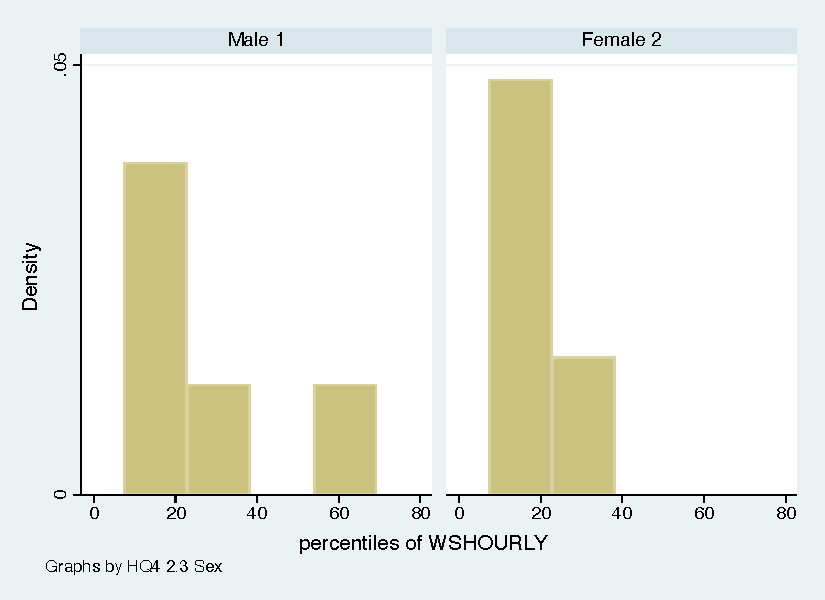
\includegraphics[width=.6\textwidth]{ps5_4.pdf}
\end{center}
The histogram of hourly wages has tails far too long to be meaningful, but this histogram grouped by decile shows the difference in the wage distribution between men and women. 
\begin{stlog}. twoway (histogram lwshourly if RO3==2, color(red)) ///
>        (histogram lwshourly if RO3==1, ///
>            fcolor(none) lcolor(blue)), legend(order(1 "Female" 2 "Male" ))
{\smallskip}
\end{stlog}
\begin{center}
    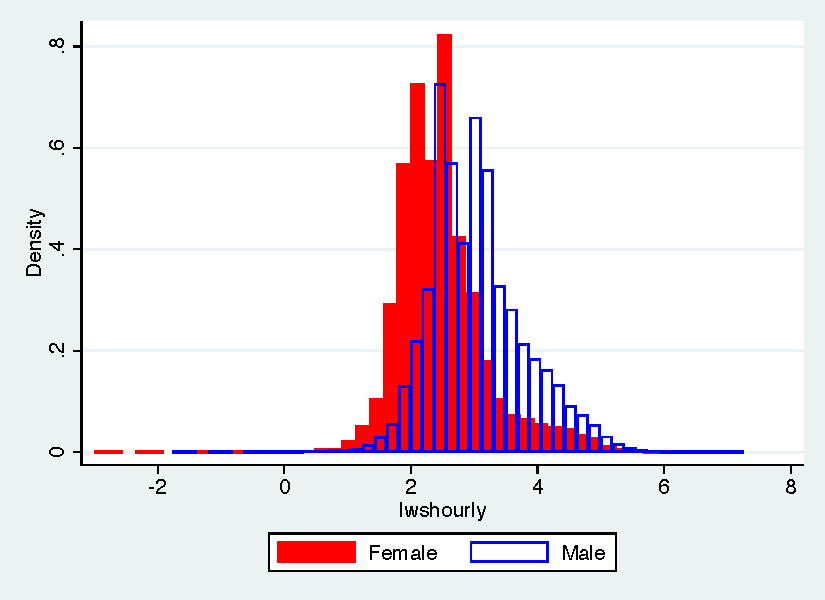
\includegraphics[width=.6\textwidth]{ps5_5.pdf}
\end{center}
This histogram shows the difference in log hourly wage distributions between men and women.

Going forward, my plan is to clean the income and wage data to get more accurate measures, including determining what to do with outliers and negative results. Then, I will construct control variables from the relevant variables in the survey. From there, I should be able to develop a fundamental OLS model with broad controls.

Then, I will develop a household fixed effects model and investigate potential instruments for gender-equality-related independent variables.

\end{document}
